\section{Methodology of the Original Paper}
\label{sec:methodo_paper}

The study by \citet{li2019estimating} aimed to reconstruct the 3D motion of a person interacting with an object, including the position 
and applied forces, from a single RGB video. Their methodology unfolds in two principal steps. The first step involves the application of 
computer vision techniques to accurately determine the human and object poses, as well as the points of contact between them and with the 
surrounding environment. The second step solves an optimization problem, rooted in control theory principles, to fully recover 
the dynamic motion. The full pipeline can be visualized on~\cref{fig:original_pipeline}.

\begin{figure*}
    \centering
    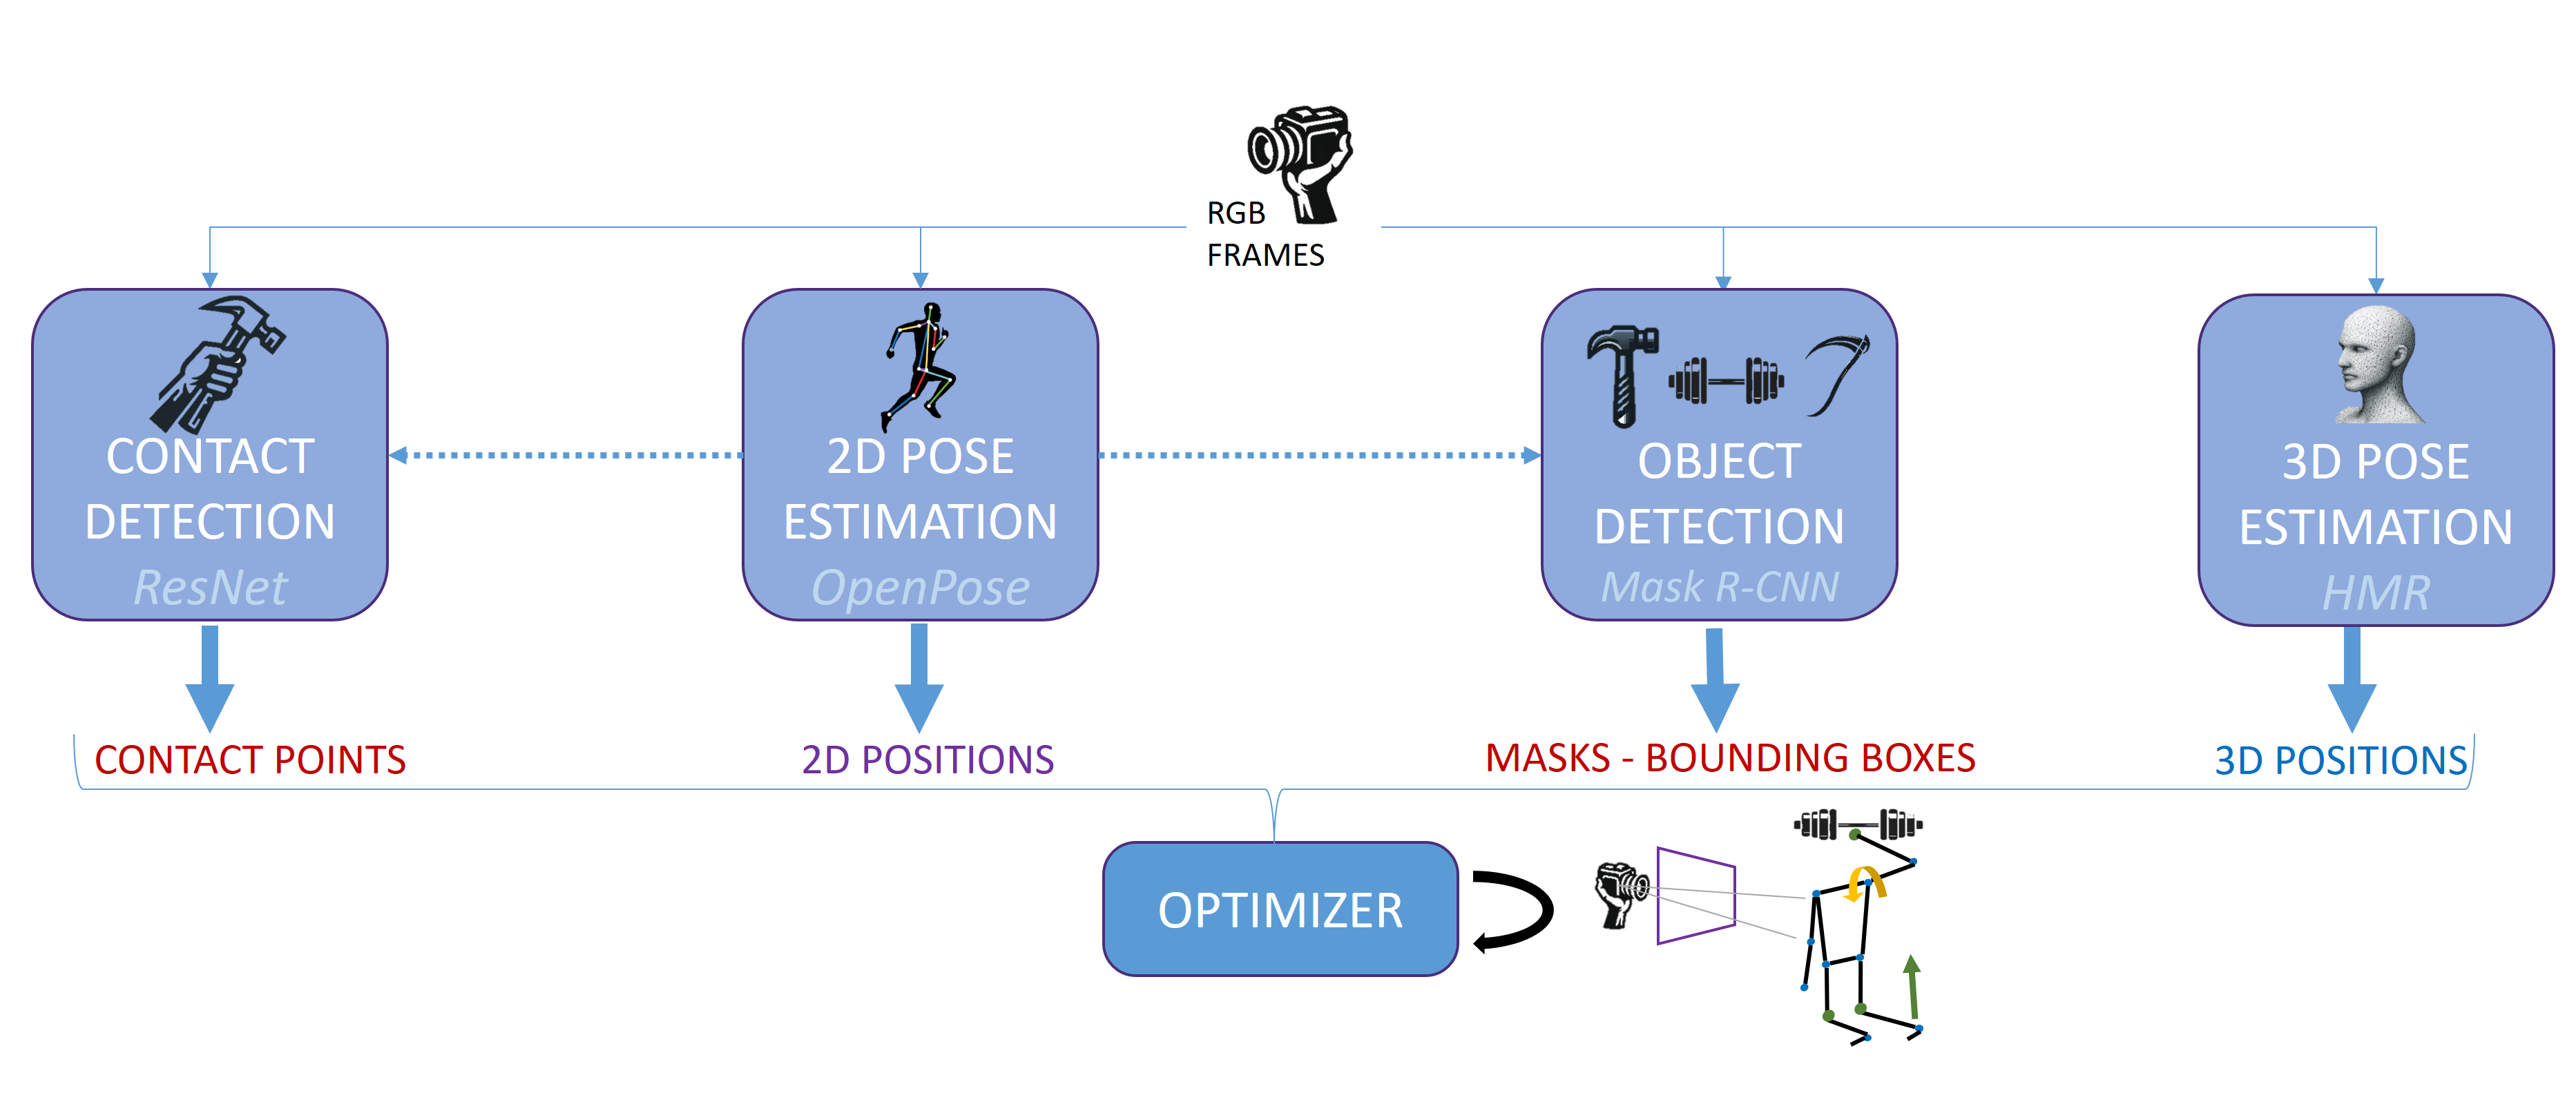
\includegraphics[width=12cm]{figures/authors_original_pipeline.png}
    \caption{Full original pipeline.}
    \label{fig:original_pipeline}
\end{figure*}


\subsection{Retrieve Human and Object 3D Pose and Contact from RGB Video}
\label{subsec:retrieve_original}

\noindent\textbf{Human 2D Pose Estimation.}\label{2dpose} For the task of human pose estimation, the authors utilized a pretrained version of 
OpenPose~\cite{cao2017realtime}. This tool enabled them to identify and track human joint positions in two dimensions from the RGB video.

\noindent\textbf{Contact Recognition.} The recognition of contact points, being whether specific joints (like feet, hands, and neck) were in 
contact with the ground or the object, was achieved by first cropping areas in the video frame around the joints identified by OpenPose. 
These cropped images were then processed through the corresponding joint's ResNet \cite{he2016deep}, which had been trained on a custom dataset 
to discern contact.

\noindent\textbf{Object 2D Endpoint Detection.} For estimating the 2D positions of object endpoints, the authors utilized instance segmentation 
capabilities of Mask R-CNN \cite{he2017mask}. This method was applied to different classes of objects (such as barbells, hammers, scythes, 
and spades) identified in their video dataset. Mask R-CNN, trained separately for each object class, enabled the extraction of segmentation masks
and bounding boxes from the video frames. These were then used to estimate the 2D locations of the object's endpoints.

\noindent\textbf{Human 3D Pose Estimation.} The authors also utilized HMR~\cite{kanazawa2018end} for 3D human pose estimation, although this 
is not clearly stated in their method overview.


\subsection{Reconstruct Person-Object Dynamic Motion}
\label{subsec:reconstruct_original}

The optimization framework presented by \citet{li2019estimating} is designed to estimate the 3D trajectories of both the human and the object, 
as well as the applied contact forces, by solving the following trajectory optimization problem: 

\begin{equation*}
    \begin{aligned}
        & \underset{x,u,c}{\text{minimize}}
        & & \int_{0}^{T} l^h(x, u, c) + l^o(x, u, c)dt, \\
        & \text{subject to}
        & & \kappa(x, c) = 0 \quad (\text{contact motion model}), \\
        &&& \dot{x} = f (x, c, u) \quad (\text{full-body dynamics}), \\
        &&& u \in \mathcal{U} \quad (\text{force model}).
    \end{aligned}
\end{equation*}

\noindent\textbf{Variables.} The state variables \(x \coloneqq (q^h, q^o, \dot{q}^h, \dot{q}^o)\) encompass the configuration and velocities of 
the human and object, while the control variables \(u \coloneqq (\tau_m^h, f_k, k=1, \dots, K)\) include the muscle torques and contact forces 
at the \(K\) contact points. The contact state \(c\) represents the presence and locations of contacts throughout the video sequence. 

It should be noted, although not explicitly stated in the paper, that in their implementation, the velocities (\(\dot{q}^h\) and \(\dot{q}^o\))
are not directly used as variables. Instead, velocities are approximated using the backward finite difference scheme 
\(\dot{q}_t = (q_t - q_{t - 1}) / \Delta t\).

\noindent\textbf{Loss Functions.} The loss functions \(l^h\) for the human consists of the following components:

\begin{itemize}
    \item 
        \(l_{2D}\): A term ensuring 2D consistency by minimizing the error between the observed 2D joint positions given by OpenPose and 
        their re-projections from the 3D estimates, using the camera projection matrix \(P_{\text{cam}}\). Outlier influence is mitigated 
        by employing the Huber loss function \(\rho\).
    \item 
        \(l_{3D}\): This loss ensures that the estimated 3D positions adhere closely to the HMR 3D references.
    \item 
        \(l_{\text{pose}}^h\): A likelihood term for the human pose, encouraging plausible human poses through a Gaussian Mixture Model 
        trained on motion capture data.
    \item
        \(l_{\text{torque}}^h\): A regularization term penalizing high muscle torque values to favor energy-efficient movements.
    \item 
        Motion smoothness: Terms penalizing rapid movements or accelerations to align with the typically smooth human motion observed over 
        the video frame rate.
    \item
        Force-related terms: These encompass additional forces and contact forces that were not the focus of further investigation in our 
        study.
\end{itemize}

The loss function for the object, \(l^o\), is constructed similarly, omitting the 3D consistency, torque smoothness and pose likelihood terms.

\noindent\textbf{Constraints.} The optimization process is subject to constraints that govern the full-body dynamics of the human and object 
interaction. These dynamics are encapsulated by the Lagrange dynamics equation:
\[
M(q)\ddot{q} + b(q, \dot{q}) = g(q) + \tau,
\]
where \( M(q) \) is the generalized mass matrix, \( b(q, \dot{q}) \) represents the centrifugal and Coriolis forces, \( g(q) \) is the 
generalized gravity vector, and \( \tau \) denotes the joint torque contributions. Here, \( \dot{q} \) and \( \ddot{q} \) are the joint 
velocities and accelerations, respectively. This constraint ensures that the estimated motion adheres to the fundamental principles of physics 
governing movement.

Other constraints, such as those related to contact, are not the focus of our study and thus are not elaborated upon here.

\noindent\textbf{Implementation.} The authors approached the problem's solution by discretizing it and applying finite difference schemes 
for derivatives, specifically \(\dot{y}_t = (y_t - y_{t - 1}) / \Delta t\). The computation of kinematic and dynamic quantities was facilitated 
by the Pinocchio library~\cite{carpentier2019pinocchio}. Optimization was performed using the Levenberg-Marquardt algorithm, within the Ceres 
Solver~\cite{Agarwal_Ceres_Solver_2022}. Due to the limitations on the constraint's type in such solvers, the constraints were incorporated as 
penalty terms in the objective function.